%%%%%%%%%%%%%%%%%%%%%%%%%%%%%%%%%%%%%%%%%
% Stylish Article
% LaTeX Template
% Version 2.2 (2020-10-22)
%
% This template has been downloaded from:
% http://www.LaTeXTemplates.com
%
% Original author:
% Mathias Legrand (legrand.mathias@gmail.com) 
% With extensive modifications by:
% Vel (vel@latextemplates.com)
%
% License:
% CC BY-NC-SA 3.0 (http://creativecommons.org/licenses/by-nc-sa/3.0/)
%
%%%%%%%%%%%%%%%%%%%%%%%%%%%%%%%%%%%%%%%%%

%----------------------------------------------------------------------------------------
%	PACKAGES AND OTHER DOCUMENT CONFIGURATIONS
%----------------------------------------------------------------------------------------

\documentclass[fleqn,10pt]{SelfArx} % Document font size and equations flushed left

\usepackage[english]{babel} % Specify a language



%----------------------------------------------------------------------------------------
%	COLUMNS
%----------------------------------------------------------------------------------------

\setlength{\columnsep}{0.55cm} % Distance between the two columns of text
\setlength{\fboxrule}{0.75pt} % Width of the border around the abstract

%----------------------------------------------------------------------------------------
%	COLORS
%----------------------------------------------------------------------------------------

\definecolor{color1}{RGB}{0,0,90} % Color of the article title and sections
\definecolor{color2}{RGB}{0,20,20} % Color of the boxes behind the abstract and headings

%----------------------------------------------------------------------------------------
%	HYPERLINKS
%----------------------------------------------------------------------------------------

\usepackage{hyperref} % Required for hyperlinks

\hypersetup{
	hidelinks,
	colorlinks,
	breaklinks=true,
	urlcolor=color2,
	citecolor=color1,
	linkcolor=color1,
	bookmarksopen=false,
	pdftitle={Title},
	pdfauthor={Author},
}

%----------------------------------------------------------------------------------------
%	ARTICLE INFORMATION
%----------------------------------------------------------------------------------------

\JournalInfo{IMT Atlantique, 14-06-2022} % Journal information
\Archive{CODEV Recherche} % Additional notes (e.g. copyright, DOI, review/research article)

\PaperTitle{Blocked Adaptive Cross Approximation (BACA)} % Article title

\Authors{KANIT Zaccarie \textsuperscript{1}*} % Authors
\affiliation{\textsuperscript{1}\textit{Étudiant en cycle d'ingénieur généraliste, IMT Atlantique}} % Author affiliation
\affiliation{*\textbf{mail}: zaccarie.kanit@imt-atlantique.net} % Corresponding author

\Keywords{Algorithme de résolution rapide -- (ML/B) ACA--Calcul Matriciel} % Keywords - if you don't want any simply remove all the text between the curly brackets
\newcommand{\keywordname}{Mots clés} % Defines the keywords heading name

%----------------------------------------------------------------------------------------
%	ABSTRACT
%----------------------------------------------------------------------------------------

\Abstract{Ce papier présente une modification de l'algorithme de calcul matricielle par ACA qui a pour objectif de réduire le temps de calcul et l'espace mémoire de la résolution des problèmes électromagnétique par la Méthode des Moments. L'algorithme proposé ici pour accélérer le calcul est l'approximation par bloc(BACA), une solution purement algébrique, qui remplace la solution par niveaux(MLACA) qui possède un manque de scalabilité. L'algorithme par bloc repose sur l'utilisation de la décomposition QR sur plus petites matrices pour améliorer la complexité. La convergence se fait donc plus rapidement et la qualité première de la ACA est maintenu; c'est à dire que l'algorithme étant purement algébrique est indépendant du noyau de Green tant que les matrices ont une déficience de rang. De plus,cet algorithme peut encore être optimisée grâce à la parallélisation de l'algorithme par bloc (H-BACA). Celui-ci étant scalable en multi coeurs et donc diminuant le temps de compilation, en particulier pour les matrices sparses.}

%----------------------------------------------------------------------------------------

\begin{document}

\maketitle % Output the title and abstract box

\tableofcontents % Output the contents section

\thispagestyle{empty} % Removes page numbering from the first page

%----------------------------------------------------------------------------------------
%	ARTICLE CONTENTS
%----------------------------------------------------------------------------------------

\section*{Introduction} % The \section*{} command stops section numbering

\addcontentsline{toc}{section}{Introduction} % Adds this section to the table of contents

La résolution rapide d'algorithme est un sujet important ces dernières année. Des algorithmes ont alors été développés pour viser des résolutions en temps réel ; il est donc nécessaire de développer des solutions plus rapides et moins couteuses en ressources.Particulièrement pour avoir des résultats instantanés dans le milieu de l'encéphalographie en résolvant de façon récursive  l'équation intégral de l'électromagnétique \cite{tamayo_multilevel_2011}. Les algorithmes de décomposition et compression de matrices peuvent alors aider à résoudre des équations de façon numérique assez rapidement. Surtout que dans ce domaine pour avoir une bonne précision il est nécessaire de stocker les informations pour de nombreuses électrodes dans des matrices $m \times n$, où $m$ et $n$ représentent la taille du grillage utilisé pour modéliser l'espace de travail. Toutefois, malgré ce nombre potentiel d'informations, les matrices utilisées peuvent souffrir d'insuffisance de rang. Malgré cela, les algorithmes naïfs comme la SVD a un coup dû à sa complexité en $\mathcal{O}(n^3)$ \cite{bebendorf_hierarchical_2008}. C'est pourquoi des algorithmes plus efficaces ont été développés; comme la ACA \cite{zhao_adaptive_2005} en premier lieu qui a donnée naissance à de nombreux algorithmes de résolution algébrique qui permettent la résolution d'équation sans connaître le noyau de la fonction de Green au préalable (pour une grande partie des fonctions de Green) \cite{bebendorf_hierarchical_2008}. De nombreux algorithmes algébriques ont alors été développé pour améliorer 

%------------------------------------------------

\section{Méthode}
\subsection{Documentation}
\subsection{Matériel}
\subsection{Procédures}


%------------------------------------------------

\section{État de l'art}
\subsection{La ACA}
\subsubsection{Présentation de l'algorithme}
\subsubsection{Analyse du coût}
\subsection{La MLACA}
\subsubsection{Présentation de l'algorithme}
\subsubsection{Analyse du coût}


%------------------------------------------------

\section{Approximation par blocs}
\subsection{Algorithme}
\subsection{Parallélisation}
\subsection{Analyses du coût}

%------------------------------------------------

\section*{Conclusion}

\addcontentsline{toc}{section}{Conclusion} % Adds this section to the table of contents


%------------------------------------------------

\section{Exemples}

\begin{figure*}[ht]\centering % Using \begin{figure*} makes the figure take up the entire width of the page
	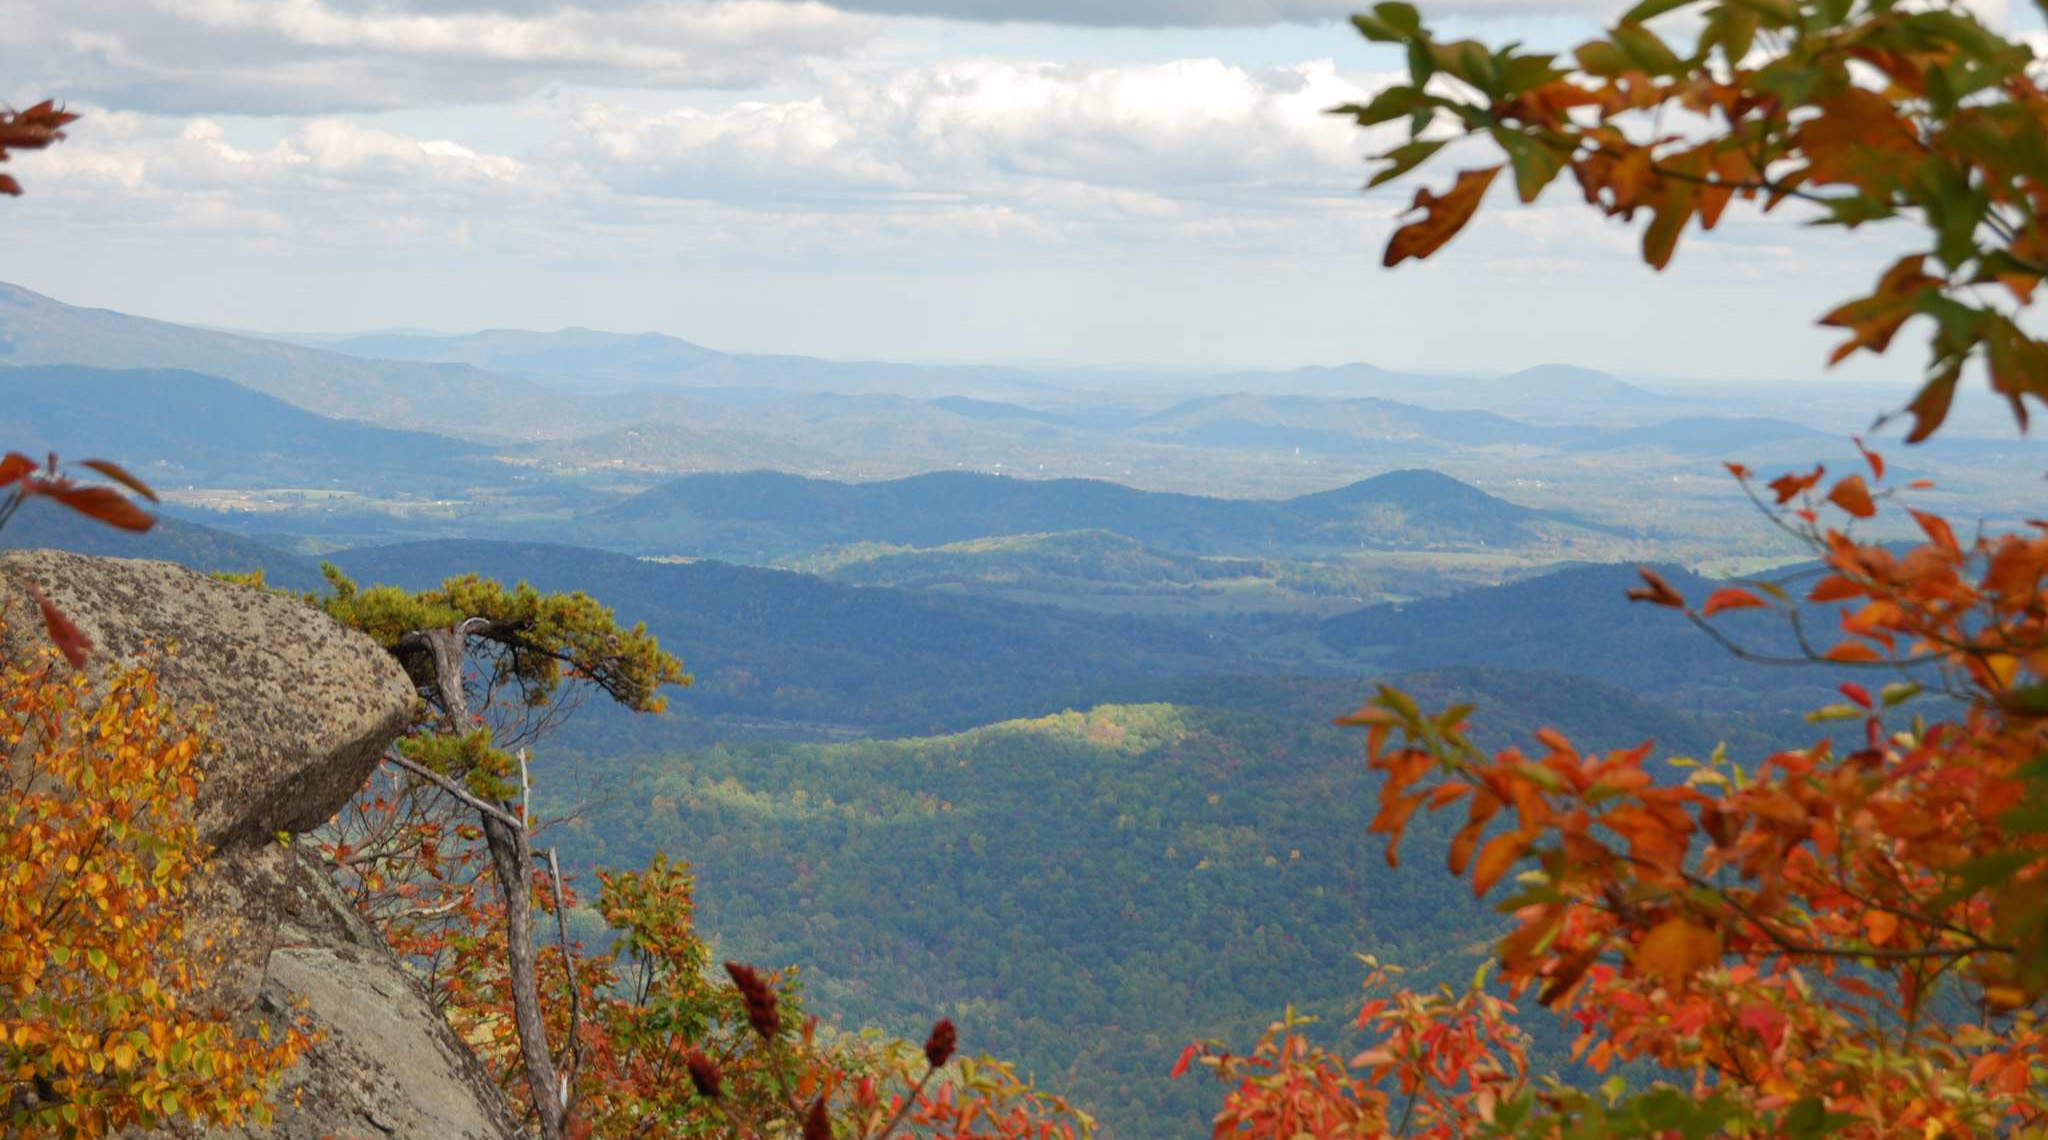
\includegraphics[width=\linewidth]{view}
	\caption{Wide Picture}
	\label{fig:view}
\end{figure*}



\begin{equation}
	\cos^3 \theta =\frac{1}{4}\cos\theta+\frac{3}{4}\cos 3\theta
	\label{eq:refname2}
\end{equation}

jhqvzjdqdq

\begin{enumerate}[noitemsep] % [noitemsep] removes whitespace between the items for a compact look
	\item First item in a list
	\item Second item in a list
	\item Third item in a list
\end{enumerate}

\subsection{Subsection}

ckjhqghd

\paragraph{Paragraph} kcjqshfdhbqd
\paragraph{Paragraph} qkjfdqhd

\subsection{Subsection}

qkbdkjhQZD

\begin{figure}[ht]\centering
	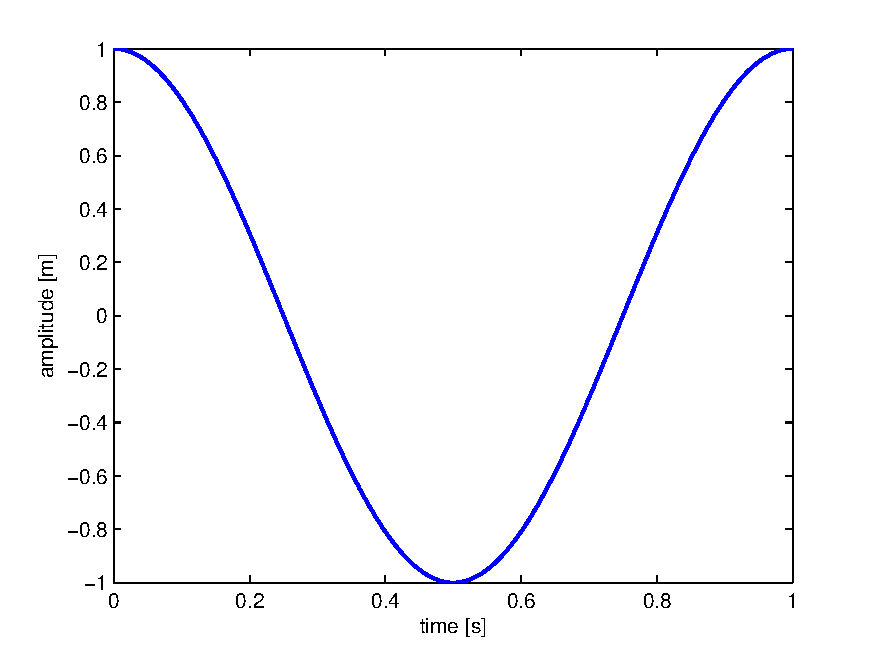
\includegraphics[width=\linewidth]{results}
	\caption{In-text Picture}
	\label{fig:results}
\end{figure}

Reference to Figure \ref{fig:results}.

%------------------------------------------------

\section{Results and Discussion}

qzjhdgqd

\subsection{Subsection}

qkjhgdvq

\begin{table}[hbt]
	\caption{Table of Grades}
	\centering
	\begin{tabular}{llr}
		\toprule
		\multicolumn{2}{c}{Name} \\
		\cmidrule(r){1-2}
		First name & Last Name & Grade \\
		\midrule
		John & Doe & $7.5$ \\
		Richard & Miles & $2$ \\
		\bottomrule
	\end{tabular}
	\label{tab:label}
\end{table}

\subsubsection{Subsubsection}

kqJDGVZkdg

\begin{description}
	\item[Word] Definition
	\item[Concept] Explanation
	\item[Idea] Text
\end{description}

\subsubsection{Subsubsection}

kqzgdkgdkgzq

\begin{itemize}[noitemsep] % [noitemsep] removes whitespace between the items for a compact look
	\item First item in a list
	\item Second item in a list
	\item Third item in a list
\end{itemize}

\subsubsection{Subsubsection}

QJHSDKQGZ

\subsection{Subsection}

lkgjqlrg
%------------------------------------------------

\phantomsection
\section*{Acknowledgments} % The \section*{} command stops section numbering

\addcontentsline{toc}{section}{Acknowledgments} % Adds this section to the table of contents

So long and thanks for all the fish. \cite{OC_obj}

%----------------------------------------------------------------------------------------
%	REFERENCE LIST
%----------------------------------------------------------------------------------------

\phantomsection
\section*{Bibliographie}

\bibliographystyle{unsrt}
\bibliography{bibli_CODEV}

%----------------------------------------------------------------------------------------

\end{document}